This chapter will summarize most of the process of creating the \gls{pcb} used to mount all the sensors and sending the data to the phone application. This circuit board will be the link between the physical forces and manipulated data sent to the handheld device. More on how this data is manipulated and how the circuit board is programmed in \autoref{sec:sw}. 

The circuit board must minimally fulfill the following set of basic requirements to function properly:
\begin{itemize}[noitemsep]
\item Circuit must fit within the casing, with dimensions extracted directly from the cad software\cite{cad}, see \autoref{fig:casdim}.
\item Circuit must be easy to test for both hardware and software errors. Even complete system needs this, since many of the sensors are very small and difficult to solder.
\item All sensors must fit on the \gls{pcb}, both physically and also electronically on the ports of the \gls{mcu}.
\item Must be protected against all common problems, such as overcharge, undercharge, capacitive effects, and more.
\item All components needs to be actively manufactured to ensure unit can keep being produced for several years in the future.
\end{itemize}

\subsection{Method}
\chapterauthor{Brolin, Daniel (Eriksson, Kenny)}
% Methodology
The main circuit board is built using the open source electronic design software \emph{KiCad}\cite{kicad}. It is completely free to use and the source code is open for any modifications.
Designing circuit boards differs slightly between what software you are using. \emph{KiCad} uses a four step process as follows:
\begin{enumerate}[noitemsep]
\item Draw schematic:
	\begin{enumerate}[noitemsep]
	\item Place and connect all components.
	\item (Optional:) All non-standard components must be custom designed, this is referred to as ``library''. Most sensors requires custom built libraries.
	\item Annotate schematic and run \gls{erc} to identify simple electronic violations.
	\end{enumerate}
\item Create net-list:
	\begin{enumerate}[noitemsep]
	\item (Optional:) All components with non-standard (or simply not standard enough) footprints must be custom designed, these include all sensors and the \gls{bt} module.
	\item Associate all components with whatever physical footprint are to be used.
	\item Generate net-list.
	\end{enumerate}
\item Design \gls{pcb} layout:
	\begin{enumerate}[noitemsep]
	\item Import net-list to \gls{pcb} editor.
	\item Set global and net-specific design rules.
	\item Place and connect all components.
	\item Run \gls{drc} to identify all specified design rule violations.
	\end{enumerate}
\item Generate manufacturing (gerber/drill) files.
\end{enumerate}
% Borrowed shit
The initial required circuitry, see \autoref{fig:schr3a}, was copied from earlier works with the \gls{st} \gls{arm} \gls{mcu}'s but modified to meet our needs. The power section, also found in \autoref{fig:schr3a}, is designed to only allow for exactly $+5V$. This design is credited to, and derived from \emph{Maxim Integrated}, Application note 760\cite{overprotection}.

% Original custom shit
Non-standard library entries include following components:\\
\begin{minipage}{\linewidth}
\begin{table}[H]
\centering
	\begin{tabular}{ l | l | l | l }
 	Name		& Type 								& Library 				& Used in         \\
 			&									&					& last rev.\footnote{revision}\\
	\hline
  	A2235-H  	& \gls{gps} 								& a2235-h.lib 			& \textbf{YES}\\
  	FT232RL 	& USBtoSerial converter 						& ftdi.lib\cite{ftdi}			& \textbf{YES}\\
  	HTS221 	& Humidity sensor 							& Custom\_sensors.lib 		& \textbf{YES}\\
  	LM1117ADJ 	& Voltage Regulator						& PowerSupply.lib\cite{lm1117} 	& \textbf{YES}\\
  	LPS22HB 	& Pressure sensor  							& Custom\_sensors.lib 		& \textbf{YES}\\
  	LSM303AGR	& Acc.\footnote{Accelerometer}/Mag.\footnote{Magnetometer} \gls{imu} & Custom\_sensors.lib & \textbf{YES}\\
  	LSM303Cx 	& Acc./Mag. \gls{imu} 						& Custom\_sensors.lib		& \textbf{NO} \\
  	LSM6DSL 	& Acc./Gyro.\footnote{Gyroscope} \gls{imu} 			& Custom\_sensors.lib 		& \textbf{YES}\\
  	LSM9DS1 	& Acc./Gyro./Mag. 							& Custom\_sensors.lib 		& \textbf{NO} \\
  	MCDTS2-4N 	& Tactile switch button 						& Custom\_Switches.lib 		& \textbf{YES}\\
\end{tabular}
\caption{Non-standard library entries custom or third-party designed.}
\label{table:nstdlibs}
\end{table}
\end{minipage}
\vspace{.5cm}

%\subsection{Revisions}\label{sec:hw:rev}
In total three revisions of the \gls{pcb} was designed. The first revision was designed well before any components arrived and was meant exclusively as a prototype, while both the second and third revisions were supposed to have full functionality. All revisions following the first were initially supposed to be designed as consecutive debugged states, but complete redesigns of component placings and tracing was eventually necessary.

\subsubsection{First revision}
First revision included the main functionality and test points on basically every pin in the system. It did not follow any space- or requirements and was riddled with small problems. The \emph{USB-to-Serial} converter was broken, the \gls{i2c} line was short circuited somewhere, the custom footprint for the \gls{gps} was mirrored, the \gls{bt} worked, but poorly due to interference from other circuitry and so on and so fourth. Most of this was probably because we had to design the \gls{pcb} and draw all custom made footprints before actually receiving the components. This revision was also meant as a prototype, and not enough time was put to make sure all isolation's and trace widths had well thought out values. A high-speed switching logic had been designed for the wakeup-signal to the \gls{gps}, but this was not used. The schematic of revision one has not been included in this report, as there is little to learn from it; the \gls{pcb} can however be seen as \autoref{fig:pcbr1}.
\begin{figure}[H]
	\centering
    \includegraphics[width=.8\linewidth]{Figures/pcb_rev1.jpg}
	\caption{First (1) revision circuit board.}
	\label{fig:pcbr1}
\end{figure}

\subsubsection{Second revision}
The second revision fixed all known problems, followed the space requirements and added a lot of customization. The option to toggle power source and what sensors were currently powered was added. This way the effect from individual modules could be measured. Also since it was still unclear if a combined chip for all \gls{imu}s would be added or not, space for all of them and an evaluation module was added. However, some wires was lost in the transition from revision one to two, as all net-labels in the schematic was redrawn; also the micro-\gls{usb} housing was to small for continuous use and was ripped of by our, way to strong, programmers; all of this was hot fixed and eventually the circuit board worked as expected. As with revision one, the schematic of revision two has not been included in this report, as there is little to learn from it; the \gls{pcb} can however be seen as \autoref{fig:pcbr2}.
\begin{figure}[H]
	\centering
	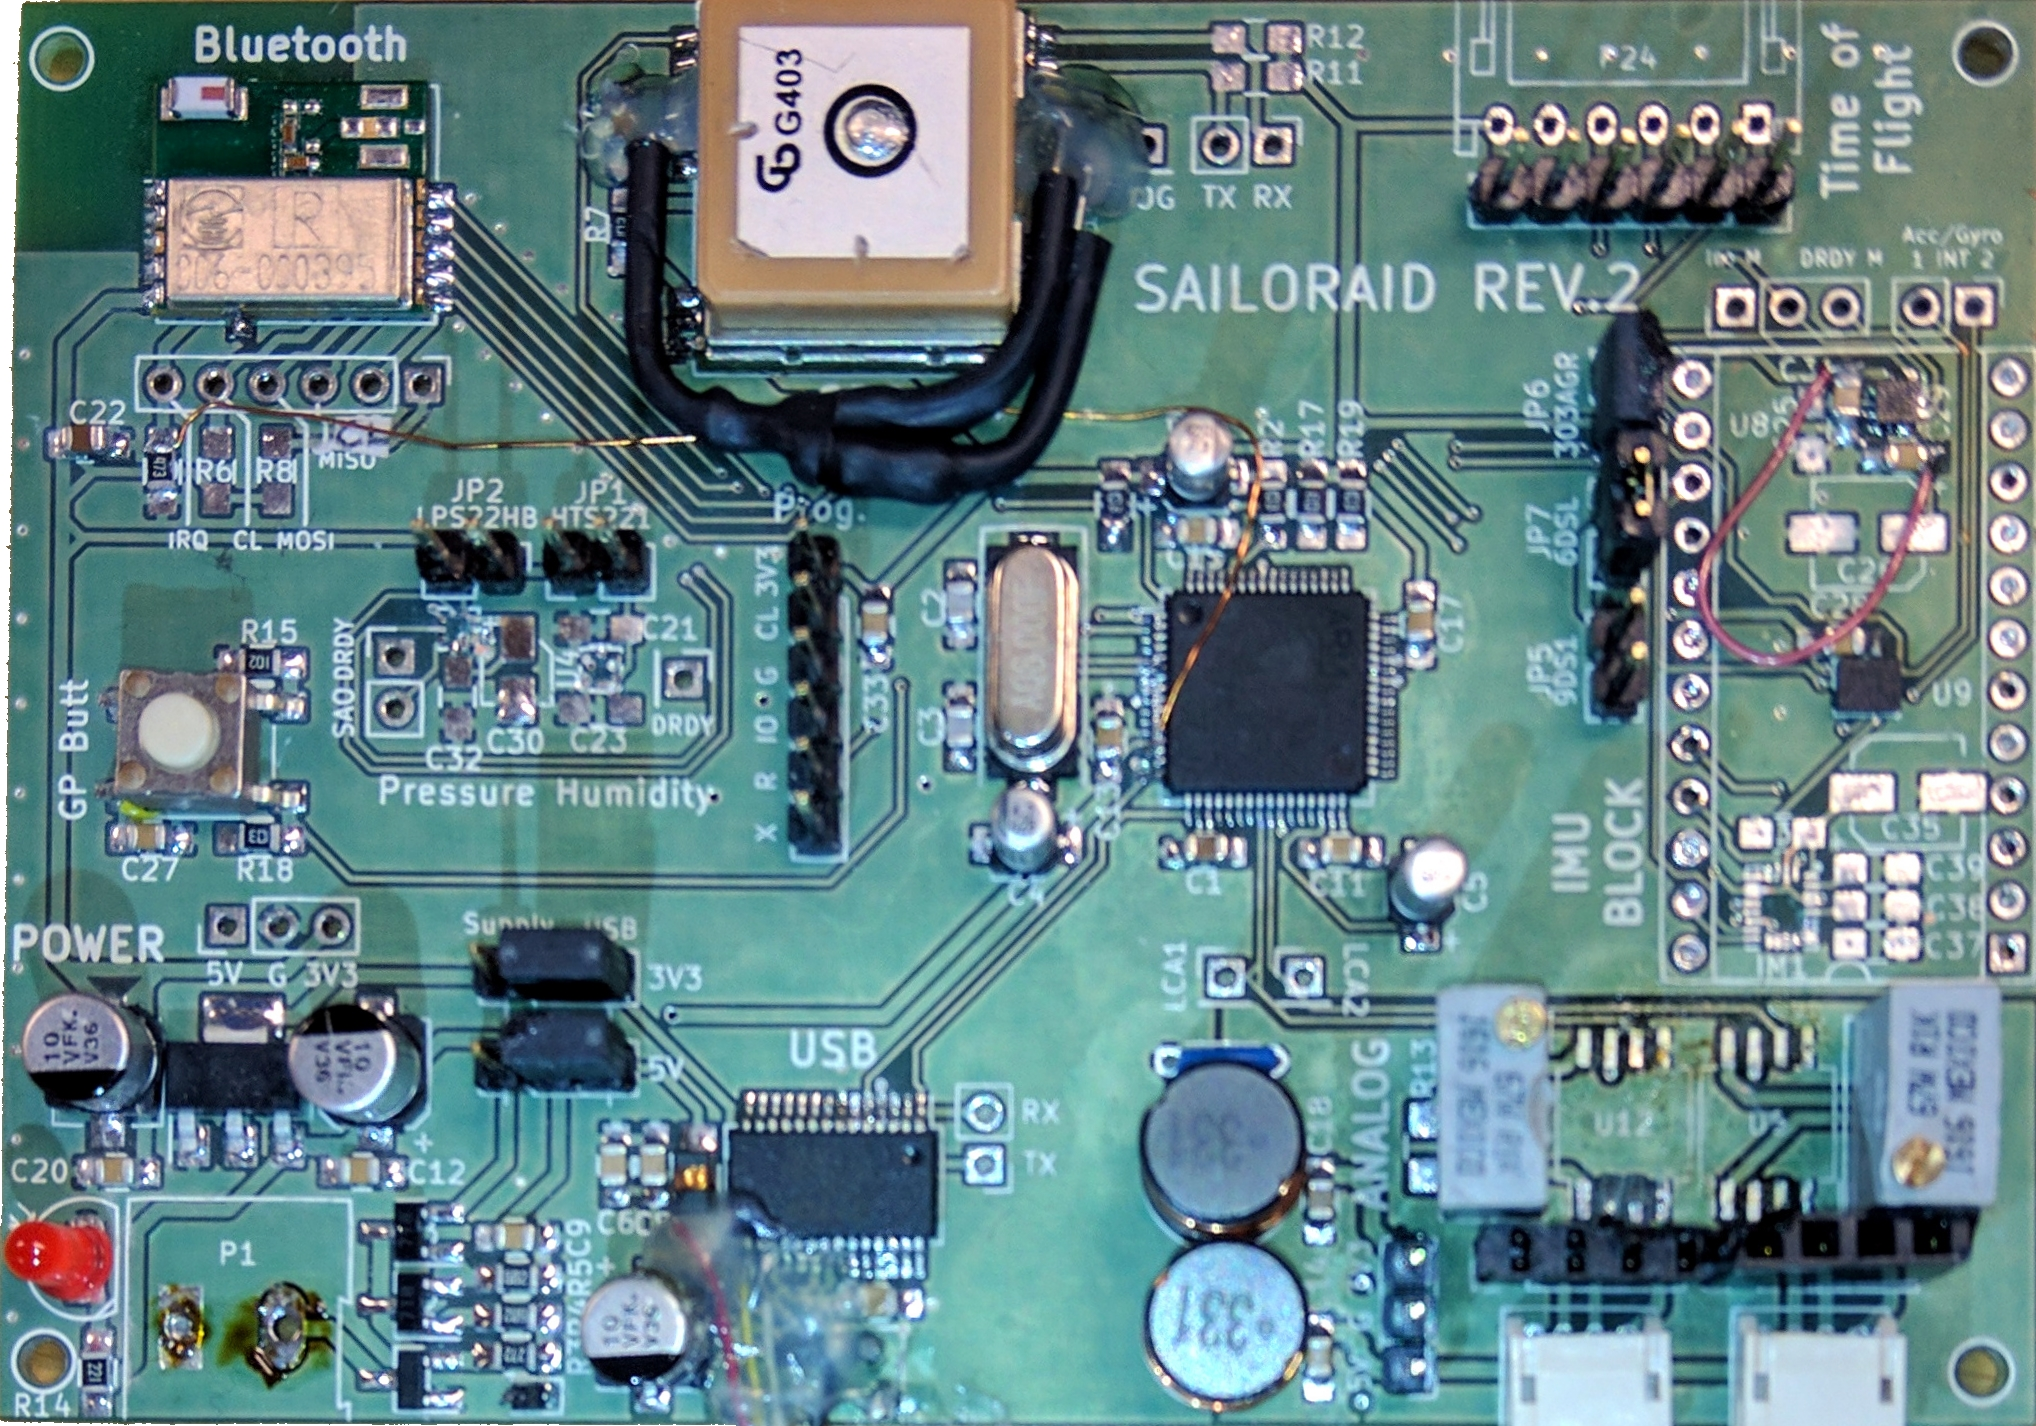
\includegraphics[width=.8\linewidth]{Figures/pcb_rev2.jpg}
	\caption{Second (2) revision circuit board.}
	\label{fig:pcbr2}
\end{figure}

\subsubsection{Third revision}
With almost all problems solved in the second revision, what remained was some hotfix for an unexpected wiring error in the \gls{gps}; interference between \gls{i2c} clock and data line; minimizing much to large decoupling ground loops; unwanted antennas; ground islands of missing copper and a KiCad problem where disconnected \gls{via}s lose their net property. The option to pull power from either \gls{usb} or batteries remained in the last revision, as this makes programming and testing much easier. A four pin connector to measure the battery level through \gls{i2c} was added; and since the power level of this depends slightly on the power left in the batteries, logic level converters was designed to allow for variable voltage levels\cite{llc}, the electronic circuitry can be see in \autoref{fig:schr3b}.
For the third revision all decisions have been made and the schematic can be seen as \autoref{fig:schr3a}, \ref{fig:schr3b} and \ref{fig:schr3c}, section \ref{app:schemmain}.

Following communicative devices will used and act as ``mudule areas'', i.e. these units will be the central units of the \gls{pcb} layout. This was introduced in the second
\begin{itemize}[noitemsep]
\item{\makebox[3cm][l]{STM32F411RET} - Microcontoller unit}
\item{\makebox[3cm][l]{FT232RL} - \gls{usb}toSerial converter (USART)}
\item{\makebox[3cm][l]{A2235-H} - \gls{gps} unit (UART)}
\item{\makebox[3cm][l]{SPBTLE-RF} - \gls{bt} connection unit (SPI)}
\item Sensors ($I^2C$):
	\begin{itemize}[noitemsep]
	\item{\makebox[3cm][l]{LSM303AGR} - Accelereometer \& Magnetometer}
	\item{\makebox[3cm][l]{LSM6DSL} - Accelerometer \& Gyroscope}
	\item{\makebox[3cm][l]{HTS221} - Humidity}
	\item{\makebox[3cm][l]{LPS22HB} - Pressure}
	\end{itemize}
\item Sensors, connectors only ($I^2C$):
	\begin{itemize}[noitemsep]
	\item Battery level
	\item VL530x \qquad- Time of flight
	\end{itemize}
\item{\makebox[2.5cm][l]{INA128} - Analog load cell amplifiers (ADC)}
\item{\makebox[2.5cm][l]{MCDTS2-4N} - Tactile push buttons (Pull-up/Pull-down)}
\end{itemize}
The layout of the components are such that all \gls{i2c} communicative devices are moved to one spot ensuring the shortest possible \gls{i2c} data line, these are placed to the top right of the \gls{pcb}. The power is placed in the bottom left, since this is as far as possible from everything else. \gls{usb} is placed next to the power, as power can be opted to be drawn from \gls{usb} rather than battery. Analog plane with the load cells are put right next to the power to ensure the star-ground\footnote{A common node ground connecting all grounds together to ensure the same set working level} to be as close as possible to the power-source allowing for as little noise as possible. \gls{bt} communication devices are rather fragile, it is therefore placed as far as possible from everything in the top left corner of the \gls{pcb}. This \gls{bt} module, \emph{SPBTLE-RF}, requires \gls{spi} communication and in total $6$ isolated traces are to be drawn between the \gls{mcu} and the \gls{bt} unit. To minimize crossover the \gls{gps} is placed in the top-mid of the \gls{pcb}. Lastly the buttons whose placing is of low importance are placed in the middle-left, between the power source and the \gls{bt} unit. 
Ground \gls{via}s was added around communication traces to prevent unwanted interference, ground \gls{via}s were also added to prevent antennas\footnote{Antennas appear by letting isolated thin grounds be connected on only one end, a \gls{via} can therefore be added to the other end to prevent this from happening.}.
The third, and last, revision of the \gls{pcb} can be seen in \autoref{fig:pcbr3}, a simple explanation of the layout can be seen in \autoref{fig:pcbr3simple}.
\begin{figure}[H]
	\centering
    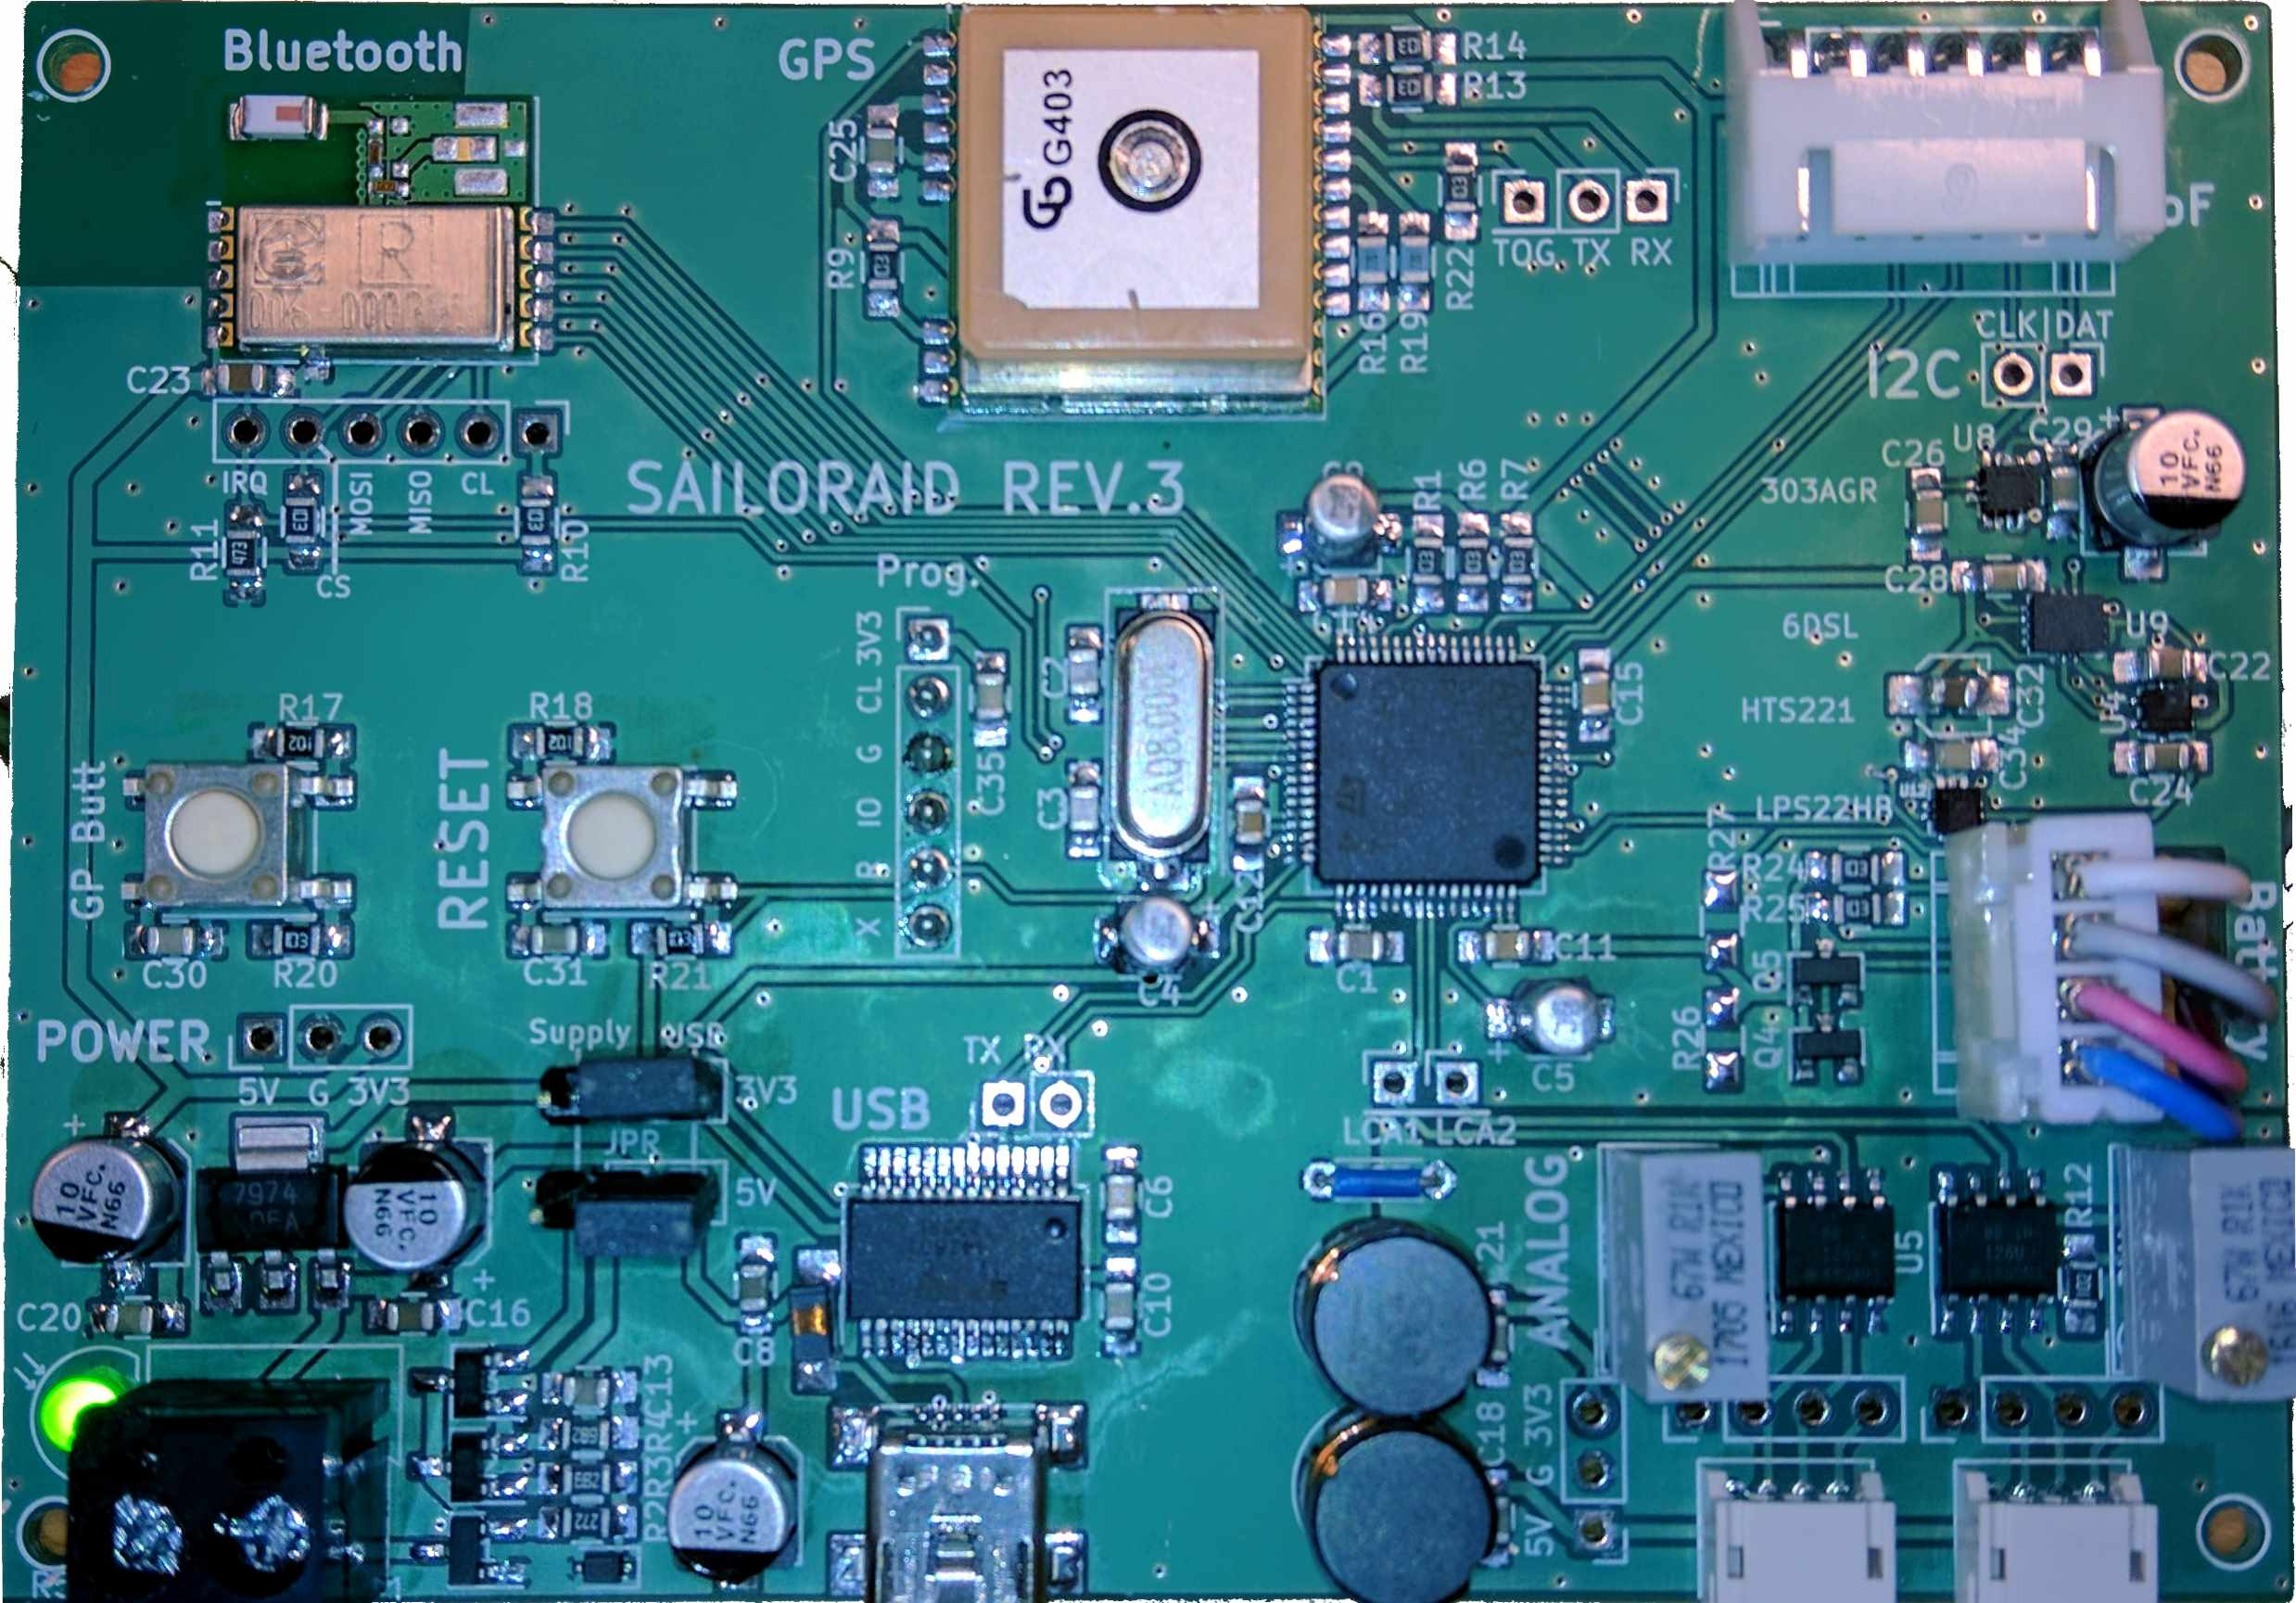
\includegraphics[width=.8\linewidth]{Figures/pcb_rev3.jpg}
	\caption{third (3) revision circuit board.}
	\label{fig:pcbr3}
\end{figure}
\begin{figure}[H]
	\centering
    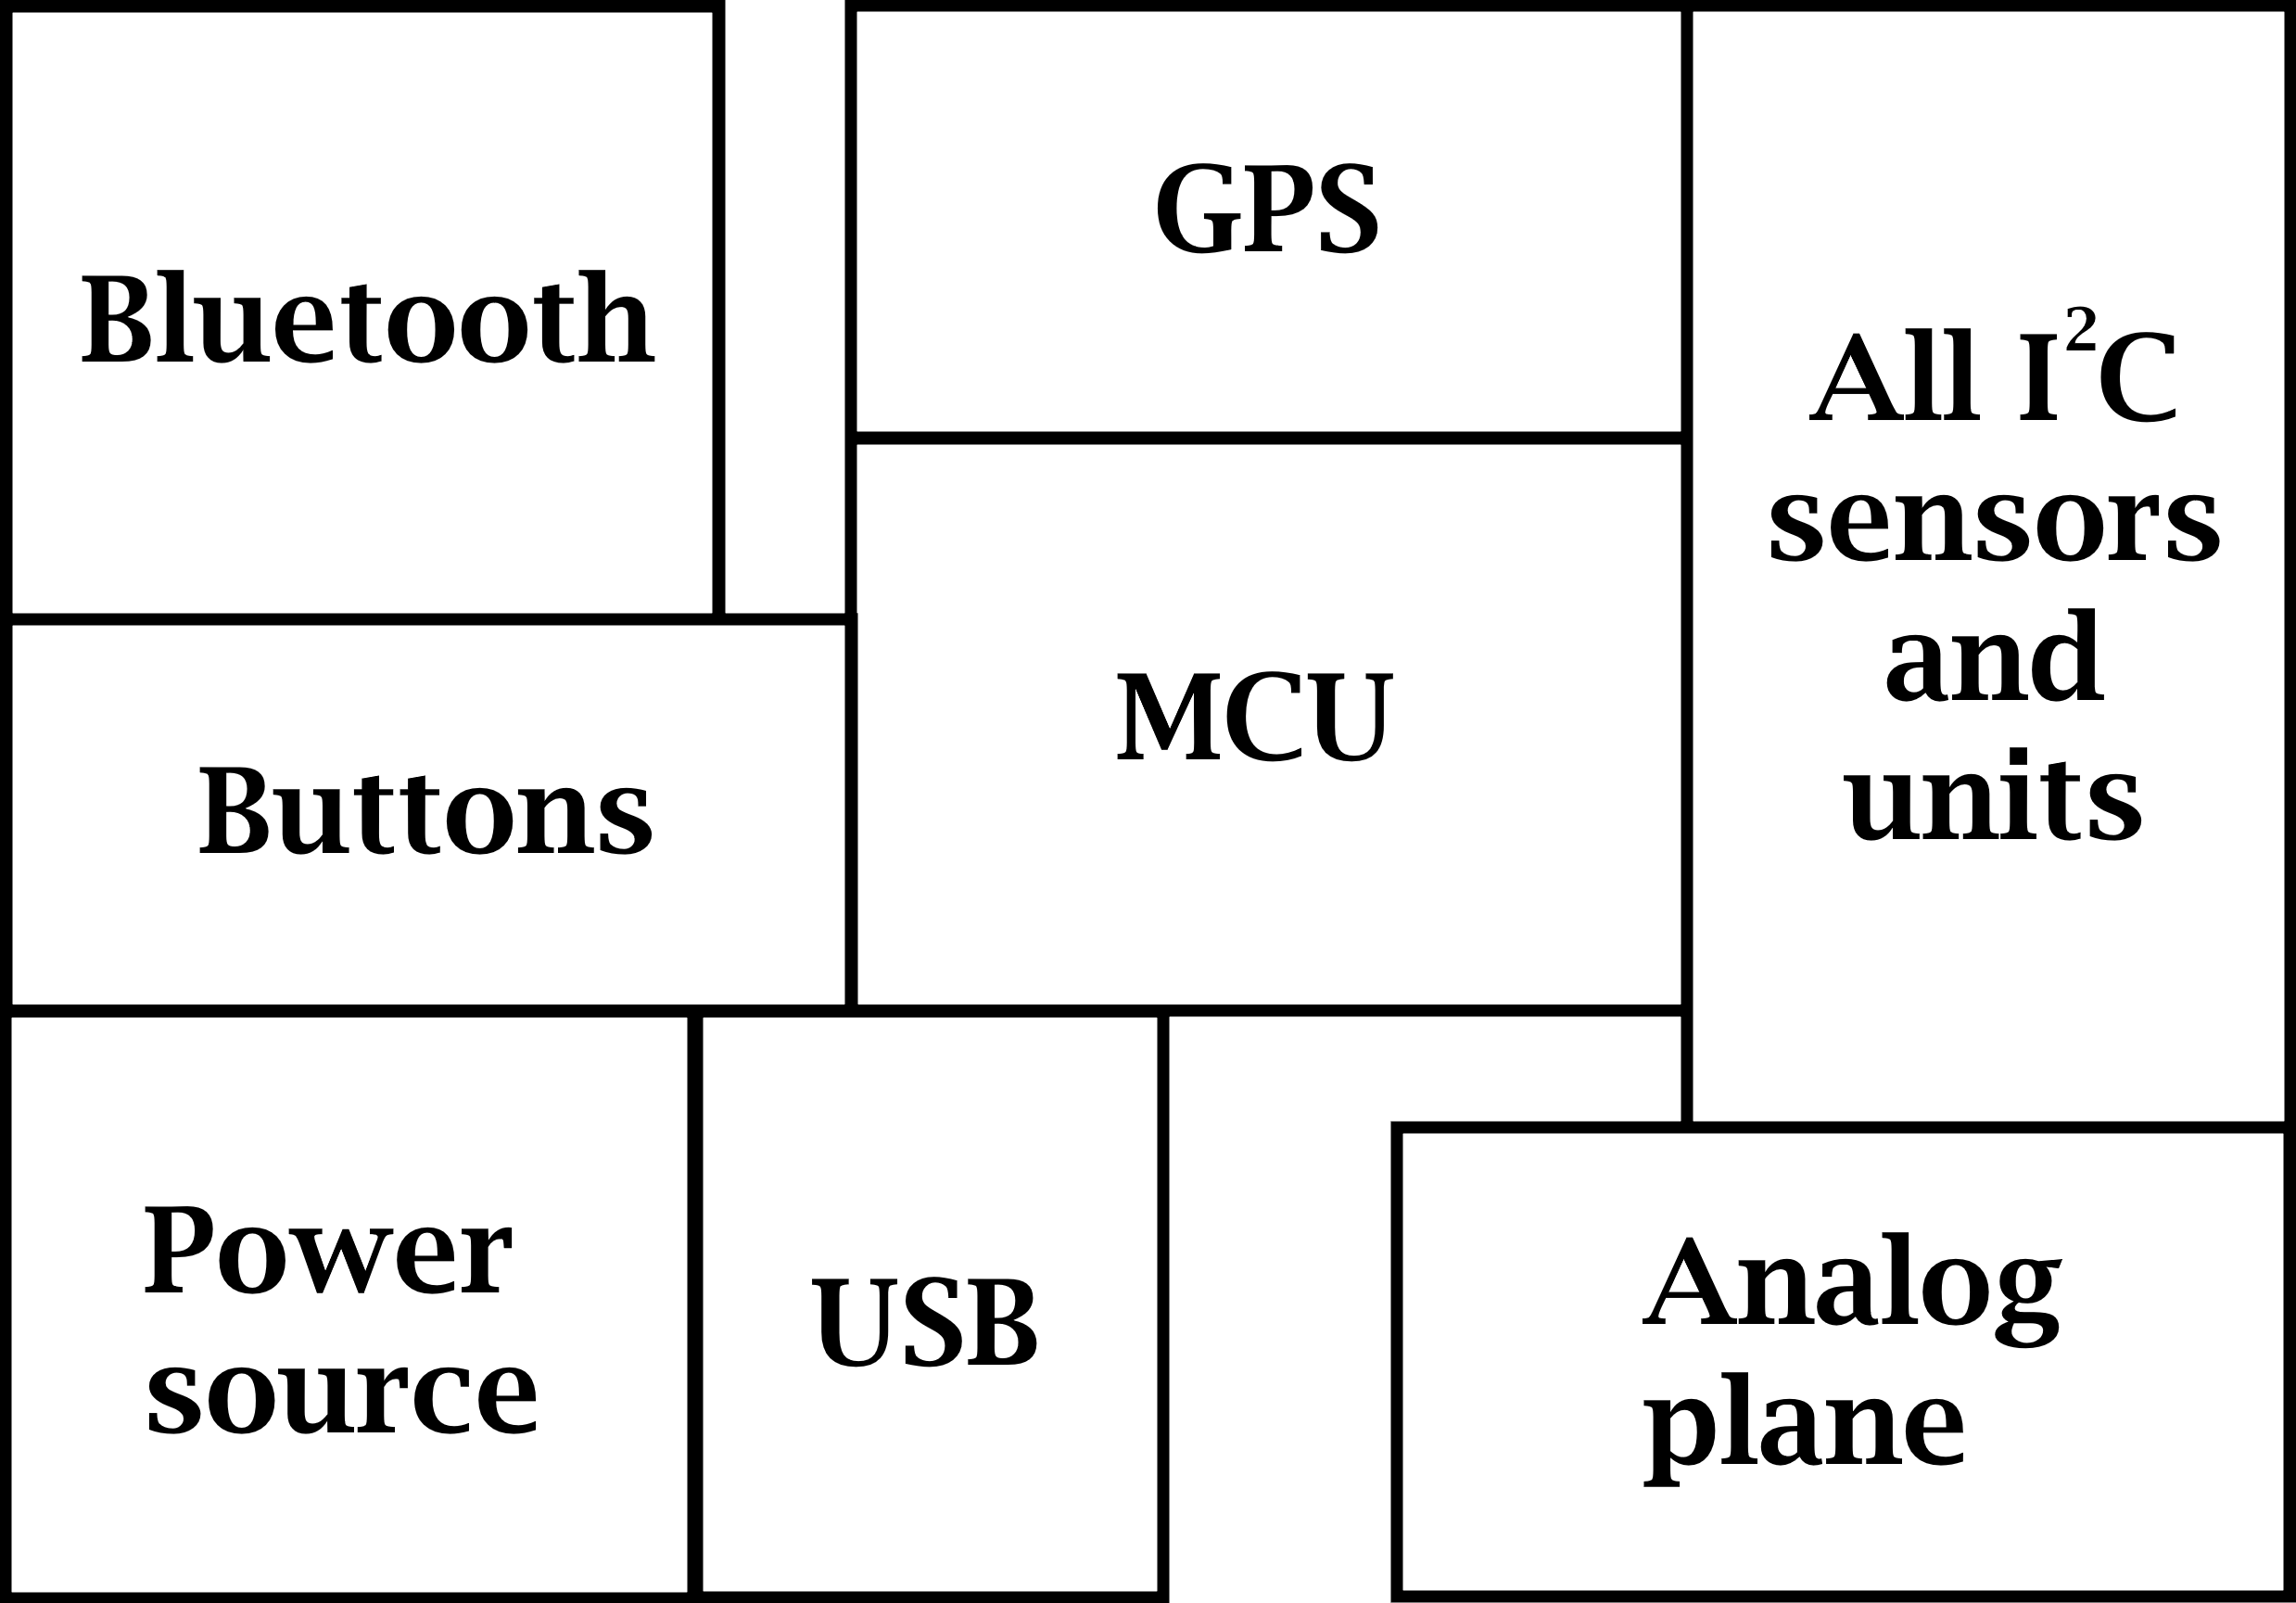
\includegraphics[width=.6\linewidth]{Figures/pcb_rev3_simple.png}
	\caption{Simple model of third (3) revision circuit board areas.}
	\label{fig:pcbr3simple}
\end{figure}

\subsection{Component choices}\label{sec:hw:tip1}
\chapterauthor{Eriksson, Kenny (Brolin, Daniel)}
In order to choose what components would be used for the system, the first consideration was the central controller of the system. Because the system was designed to work in conjunction with an app on a smartphone it was agreed that there is no need for heavy computation on the on-board module. This meant that a \gls{mcu} would be sufficient. Because several of the project members had previous experience with the \gls{st} brand \emph{STM32F411RE} and it has a significant number of GPIO ports, useful peripherals (\gls{i2c}, \gls{spi}, timers, etc) and a high clock speed of up to $100~\textrm{MHz}$ it was chosen as the core of the on-board module. 

The \emph{STM32F411RE} utilizes the \gls{swd} protocol for programming and debugging, the programmer in this case being the programming section of a \emph{NUCLEO-F411RE} development board configured as a programmer. The \gls{swd} header also provides a \gls{uart} channel to communicate with the \gls{mcu}. However, in the interest of convenience for the developers a \emph{FT232RL} chip was added. The \emph{FT232RL} is a \emph{\gls{usb}-to-\gls{uart}} converter that also allows for the \gls{usb} to act as a power source for the board. This eliminated the need for the prototypes to be connected to a power supply and the programmer at times when they were not necessary, giving the more convenient alternative of a common \gls{usb} cable.  The FT232RL was configured only to provide the communication conversion and the power. There are more features available to the FT232RL but no use was found as the on-board module is not connected to a \gls{usb} port for the majority of its operation. 

In order to communicate with the smartphone in a convenient way the on-board module used a Bluetooth module, the SPBTLE-RF. It was chosen as a compact complete module, eliminating the need for soldering inconvenient components and designing \gls{pcb} antennas, and because ST Microelectronics provide official libraries for the \emph{STM32F411RE-to-SPBTLE-RF} interface. 

One of the primary functions that the system had to provide was velocity. The velocity is derived from the position of the boat as measured with \gls{gps}. This necessitated a \gls{gps} module. The project group from the previous year had thought the same thing, and among the remains of their project was a \emph{A2235-H} module. The \emph{A2235-H} module fit the requirements of the project, as it provided circa 1Hz update rate with sub-meter precision in reasonable conditions, all within a compact form factor. It did however have some requirements on how it could be initialized, otherwise risking corruption of the \gls{gps} modules firmware. 

The second primary function the board was supposed to provide was the ability to tell the boats orientation. The common Madgwick method discussed later relies on the use of an accelerometer, magnetometer and gyroscope in conjunction. Because the \gls{mcu} had already been decided we looked for compatible development boards that had the required components and ideally also support libraries. Having found the \emph{NUCLEO-1KS01A2} that satisfies this, the components were chosen from the development board to be able to reuse already written code. 

For magnetometer, the \emph{LSM303AGR} was what was on the development board. It incorporates both an accelerometer and a magnetometer and testing the development board showed it performed good enough for the intended purpose. For the gyroscope, the \emph{LSM6DSL} had once again proved good enough for our purpose, and it too incorporated an accelerometer, possibly allowing for additional filtering possibilities in the future. 

During the course of the project we considered two changes to the choice of components. One was to change from the \emph{LSM303AGR} to the \emph{LSM303C} because of apparent lack of availability, but we found another place to get the already chosen part. The second change we considered was to replace the \emph{LSM6DSL} and \emph{LSM303AGR} with the \emph{LSM9DS1}, which incorporates the magnetometer, accelerometer and gyroscope in a single package to minimize the need to solder inconvenient packages, but because we could not find any official libraries we decided to not change over, so as to not have to rewrite the entire library by ourselves. 

In addition to the \gls{imu} sensors, the development board also provided two additional sensors: the \emph{HTS221}thermometer and relative humidity sensor, and the \emph{LPS22HB} pressure sensor. These were included in the final design to give room for expansion. 



\subsection{Results, Discussion and Future Work}\label{sec:hw:tip2}
\chapterauthor{Brolin, Daniel (Eriksson, Kenny)}
The final sensor board works as expected. Had it not been for the fact that one of the sensors was broken it would have been soldered without any problem. No interference problems or antennas has been found on the last revision \gls{pcb} and no hot fixes were necessary.
Calibrating the potentiometers for the analog load cell amplifiers is possibly the most uncertain process, as wrongly tuning these will offset all values in the feedback. This is however necessary until the last prototype for the casing is complete, see \autoref{sec:case}, since small differences in the casing will require different calibrations.
The system is estimated to run for about $24hrs$, more about power management in \autoref{sec:bat}. 

All components in the last revision prototype is of a rather large form factor considering the relatively low effect acting on the components, making soldering and testing easier but taking up more space. As it is now the system can very likely be minimized further. Taking away the general purpose button, set the general form factor to the industry standard $0402$ (approximately $1mm$x$.5mm$) which is still easily soldered by hand), use $4$-layer design could probably shrink the system to about half of the size if no more devices are added to the design. Alternatively more sensors or communication with an external sensor board could be supported in future updates without the need of to much remodeling. 